\chapter{Biomoléculas: aminoácidos, azúcares, lípidos y nucleótidos}\label{ch:b2:biomolecules}

Un edulcorante corriente, mucho más dulce que el azúcar, está formado por dos aminoácidos unidos por un único enlace amida, uno
de ellos en forma de éster metílico: el ácido aspártico y la fenilalanina, ambos con la configuración que usan las células
vivas. Las moléculas de la vida se construyen a partir de unas pocas familias de unidades pequeñas, aminoácidos, azúcares, \omterm{def:b2:biomolecules:lipid}{ácidos
grasos} y \omterm{def:b2:biomolecules:nucleotide}{nucleótidos}, unidas por las reacciones de los capítulos anteriores: amidas, acetales, ésteres. Este
capítulo las lee como lo hace un químico orgánico: grupos funcionales, estereoquímica, comportamiento
ácido--base, y las reacciones que las unen y las cortan.
% ledger: use:aspartame

\begin{recall}
El volumen del primer año: reglas CIP, proyecciones de Fischer, quiralidad, hemiacetales y acetales, $\mathrm pK_a$
y diagramas de distribución, moléculas anfífilas, ley de Biot. \Cref{ch:b2:acyl-substitution}: amidas,
ésteres, \omterm{def:b2:acyl-substitution:saponification}{saponificación}, ácidos activados. \Cref{ch:b2:amines}: las aminas como bases.
\Cref{ch:b2:retrosynthesis}: grupos protectores en una ruta.
\end{recall}

\section{Aminoácidos}

\begin{definition}[Aminoácidos]\label{def:b2:biomolecules:amino-acid}
Un \emph{$\alpha$-aminoácido}\index{alfa-aminoacido@$\alpha$-aminoácido} \ce{H2N-CHR-COOH} lleva un
grupo amino y un grupo ácido carboxílico sobre el mismo carbono; \ce{R} es su \emph{cadena
lateral}\index{cadena lateral}. En agua, cerca de pH neutro, existe como \emph{ion dipolar}\index{ion dipolar} (zwitterión),
\ce{H3N+-CHR-COO-}, que lleva una carga positiva y una negativa. El \emph{punto
isoeléctrico}\index{punto isoelectrico@punto isoeléctrico} pI es el pH al que su carga neta media es nula.
\end{definition}

Veinte aminoácidos construyen las proteínas de los seres vivos. Todos salvo la glicina (\ce{R = H}) son quirales, y
los naturales tienen la configuración L (\cref{def:b2:biomolecules:d-l}). Sus \omterm{def:b2:biomolecules:amino-acid}{cadenas laterales} los clasifican
en familias: apolares (alanina, \ce{R = CH3}; fenilalanina, \ce{R = CH2C6H5}), polares, ácidos
(ácidos aspártico y glutámico, con un segundo grupo carboxílico) y básicos (lisina, con un segundo grupo
amino; histidina, con un anillo de imidazol).

\begin{proposition}[Punto isoeléctrico]\label{prop:b2:biomolecules:pi}
Para un aminoácido con una \omterm{def:b2:biomolecules:amino-acid}{cadena lateral} que no es ni ácida ni básica, $\mathrm{pI} = (\mathrm pK_{a1} +
\mathrm pK_{a2})/2$, donde $\mathrm pK_{a1}$ corresponde al grupo carboxílico y $\mathrm pK_{a2}$ al
grupo amonio. Para una \omterm{def:b2:biomolecules:amino-acid}{cadena lateral} ácida o básica, el pI es la media de los dos $\mathrm pK_a$ que enmarcan la
forma neutra.
\end{proposition}

\begin{proof}
Escríbase \ce{H2A+} para el catión, \ce{HA} para el \omterm{def:b2:biomolecules:amino-acid}{ion dipolar} y \ce{A-} para el anión. La carga neta es
nula cuando $[\ce{H2A+}] = [\ce{A-}]$. De $K_{a1} = [\ce{HA}]h/[\ce{H2A+}]$ y $K_{a2} =
[\ce{A-}]h/[\ce{HA}]$, con $h = [\ce{H3O+}]$, la razón $[\ce{H2A+}]/[\ce{A-}] = h^2/(K_{a1}K_{a2})$
vale 1 para $h^2 = K_{a1}K_{a2}$, es decir, $\mathrm{pH} = (\mathrm pK_{a1} + \mathrm pK_{a2})/2$. Con un
tercer grupo ionizable, el mismo argumento se aplica a los dos equilibrios situados a ambos lados de la forma
neutra, pues el tercer grupo está entonces totalmente en un solo estado.
\end{proof}

Para la glicina, $\mathrm pK_{a1} = 2.35$ y $\mathrm pK_{a2} = 9.78$: pI $\approx 6.1$. El ácido aspártico
(2.0, 3.9, 9.9) tiene pI $\approx 3.0$; la lisina (2.2, 9.1, 10.7) tiene pI $\approx 9.9$.
% ledger: pka:glycine1, pka:glycine2, pka:asp1, pka:asp2, pka:asp3, pka:lys1, pka:lys2, pka:lys3

\begin{omfigure}
\begin{tikzpicture}
\begin{axis}[width=0.47\linewidth, height=5cm, xmin=0, xmax=14, ymin=-2.2, ymax=2.2,
  xlabel={pH}, ylabel={carga neta}, label style={font=\small}, tick label style={font=\scriptsize},
  xtick={0,2,4,6,8,10,12,14}, ytick={-2,-1,0,1,2}, grid=major, grid style={black!12},
  legend style={font=\scriptsize, at={(0.5,1.03)}, anchor=south}, legend columns=3]
\addplot[omDef, thick] table[x=pH, y=gly] {figdata/out/bachelor-2-amino-acid-charge-a.dat};
\addplot[omThm, thick] table[x=pH, y=asp] {figdata/out/bachelor-2-amino-acid-charge-a.dat};
\addplot[omMeth, thick] table[x=pH, y=lys] {figdata/out/bachelor-2-amino-acid-charge-a.dat};
\legend{glicina, ácido aspártico, lisina}
\end{axis}
\end{tikzpicture}\hfill
\begin{tikzpicture}
\begin{axis}[width=0.47\linewidth, height=5cm, xmin=0, xmax=14, ymin=0, ymax=1.05,
  xlabel={pH}, ylabel={fracción}, label style={font=\small}, tick label style={font=\scriptsize},
  xtick={0,2,4,6,8,10,12,14},
  legend style={font=\scriptsize, at={(0.5,1.03)}, anchor=south}, legend columns=3]
\addplot[omThm, thick] table[x=pH, y=cation] {figdata/out/bachelor-2-amino-acid-charge-b.dat};
\addplot[omDef, thick] table[x=pH, y=zwitterion] {figdata/out/bachelor-2-amino-acid-charge-b.dat};
\addplot[omMeth, thick] table[x=pH, y=anion] {figdata/out/bachelor-2-amino-acid-charge-b.dat};
\legend{catión, ion dipolar, anión}
\end{axis}
\end{tikzpicture}

{\small Izquierda: carga neta de tres aminoácidos en función del pH, a partir de sus $\mathrm pK_a$ a
\qty{25}{\degreeCelsius}; cada curva corta el cero en el pI. Derecha: las tres formas de la glicina,
\ce{H3N+CH2COOH}, \ce{H3N+CH2COO-} y \ce{H2NCH2COO-}; el \omterm{def:b2:biomolecules:amino-acid}{ion dipolar} predomina aproximadamente de pH 3 a
pH 9.}
% figdata: bachelor-2/amino-acid-charge.py parts a, b
\end{omfigure}

\begin{method}[Carga neta a un pH dado]\label{met:b2:biomolecules:charge}
\begin{enumerate}
  \item Enumérense todos los grupos ionizables con su $\mathrm pK_a$: el \ce{NH3+} y el \ce{COOH} terminales, y las
        \omterm{def:b2:biomolecules:amino-acid}{cadenas laterales} ionizables.
  \item Para cada grupo, compárense el pH y el $\mathrm pK_a$: un grupo está mayoritariamente protonado por debajo de su
        $\mathrm pK_a$, y mayoritariamente desprotonado por encima (a más de 1 unidad: más del 90~\%).
  \item Súmense las cargas: \ce{NH3+} $+1$, \ce{NH2} 0, \ce{COOH} 0, \ce{COO-} $-1$ (imidazolio $+1$).
  \item Cerca de un $\mathrm pK_a$, cuéntese ese grupo como medio cargado; para un valor exacto, úsense las fracciones
        $1/(1 + 10^{\mathrm pK_a - \mathrm{pH}})$.
\end{enumerate}
\end{method}

\section{Péptidos}

\begin{definition}[Péptidos]\label{def:b2:biomolecules:peptide}
El enlace amida formado entre el grupo carboxílico de un aminoácido y el grupo amino de otro es
un \emph{enlace peptídico}\index{enlace peptidico@enlace peptídico}; una cadena de aminoácidos unidos por enlaces peptídicos es un
\emph{péptido}\index{peptido@péptido} (una proteína cuando es largo), que se escribe desde su extremo amino libre (N-terminal)
hasta su extremo carboxílico libre (C-terminal). Un \emph{acoplamiento peptídico}\index{acoplamiento peptidico@acoplamiento peptídico} forma un
enlace peptídico en el laboratorio con un \emph{agente de acoplamiento}\index{agente de acoplamiento}, un reactivo que
convierte el grupo carboxílico en un derivado activado en condiciones suaves (una carbodiimida, por
ejemplo).
\end{definition}

\begin{omfigure}
\setchemfig{atom sep=1.9em}
\schemestart
\chemfig{R-C(=[2]O)-N(-[6]H)-R'}
\arrow{<->}
\chemfig{R-C(-[2]\chemabove{O}{\scriptstyle -})=\chemabove{N}{\scriptstyle +}(-[6]H)-R'}
\schemestop
\par\vspace{6pt}

{\small Las dos estructuras de resonancia del \omterm{def:b2:biomolecules:peptide}{enlace peptídico}. El par no enlazante del nitrógeno se comparte con el
carbonilo: el enlace \ce{C-N} tiene un carácter parcial de doble enlace, y los seis átomos C, C, O, N, H, C están
en un mismo plano.}
\end{omfigure}

\begin{proposition}[Un enlace plano]\label{prop:b2:biomolecules:planar}
El \omterm{def:b2:biomolecules:peptide}{enlace peptídico} es plano, la rotación en torno al enlace \ce{C-N} está restringida, y el nitrógeno de la amida no es
ni básico ni nucleófilo.
\end{proposition}

\begin{proof}[Argumento]
La segunda estructura de resonancia da al enlace \ce{C-N} una parte de carácter de doble enlace: hacerlo girar
rompería el solapamiento del par no enlazante del nitrógeno con el sistema $\pi$ \ce{C=O}, lo que cuesta energía, de modo que
los átomos que lo rodean permanecen en un mismo plano, siendo la disposición trans (los dos carbonos de la cadena a lados opuestos
del enlace \ce{C-N}) la habitual. El par no enlazante comprometido en la resonancia no está disponible para un protón ni para un
electrófilo, como en toda amida (\cref{ch:b2:acyl-substitution}). Las proteínas se pliegan en torno a cadenas de estos
planos rígidos.
\end{proof}

\begin{proposition}[Por qué proteger y activar]\label{prop:b2:biomolecules:coupling}
Obtener un dipéptido dado a partir de dos aminoácidos requiere a la vez proteger los grupos que no deben
reaccionar y activar el grupo carboxílico que sí debe hacerlo.
\end{proposition}

\begin{proof}[Argumento]
Un ácido carboxílico y una amina mezclados a temperatura ambiente dan una sal, no una amida; calentar para eliminar
el agua racemizaría además los aminoácidos. Hace falta, por tanto, una activación (un \omterm{def:b2:acyl-substitution:derivative}{cloruro de acilo}, un anhídrido o un
\omterm{def:b2:biomolecules:peptide}{agente de acoplamiento}). Pero cada aminoácido tiene ambos grupos: activar una mezcla de glicina y
alanina daría Gly--Ala, Ala--Gly, Gly--Gly, Ala--Ala y cadenas más largas. Bloquear la amina del
primero y el ácido del segundo deja un único enlace posible.
\end{proof}

\begin{method}[Síntesis de un dipéptido]\label{met:b2:biomolecules:peptide}
\begin{enumerate}
  \item Protéjase el grupo amino del aminoácido N-terminal (como carbamato, por ejemplo un
        grupo \textit{terc}-butoxicarbonilo).
  \item Protéjase el grupo carboxílico del aminoácido C-terminal (como éster metílico o bencílico), y toda
        \omterm{def:b2:biomolecules:amino-acid}{cadena lateral} reactiva.
  \item Actívese el grupo carboxílico libre con un \omterm{def:b2:biomolecules:peptide}{agente de acoplamiento} y añádase el compañero protegido: se forma un
        \omterm{def:b2:biomolecules:peptide}{enlace peptídico}.
  \item Elimínense los grupos protectores, preferiblemente un conjunto ortogonal
        (\cref{def:b2:retrosynthesis:orthogonal}); para continuar, elimínese solo la protección de la amina y repítase.
\end{enumerate}
\end{method}

Repetir el ciclo muchas veces en disolución exigiría una purificación en cada etapa. En la síntesis en fase
sólida, la cadena en crecimiento está unida por su extremo C-terminal a una perla de \omterm{def:b2:polymer-synthesis:polymer}{polímero}; los reactivos en exceso y los
subproductos se eliminan por lavado tras cada acoplamiento, y el \omterm{def:b2:biomolecules:peptide}{péptido} terminado se separa del soporte al
final.

\begin{omfigure}
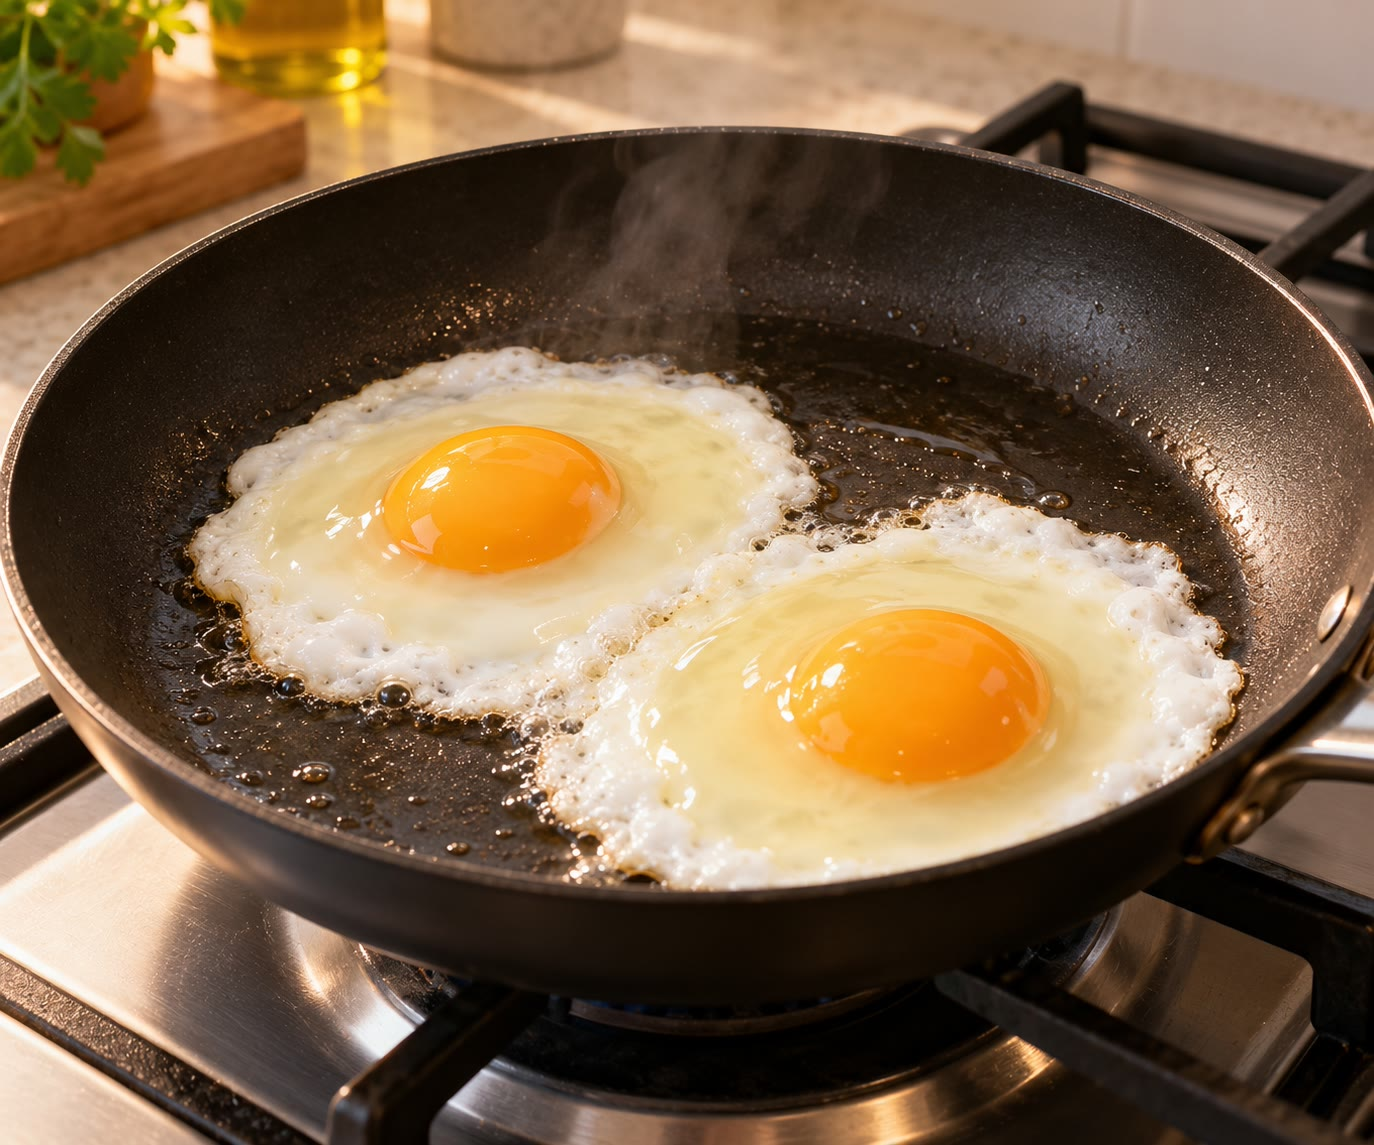
\includegraphics[width=0.5\linewidth]{images/book3/ai/b2-30-eggs.jpg}

{\small Huevos friéndose. Las proteínas de la clara se despliegan al calentarse y se unen unas con otras: el
líquido translúcido se convierte en un sólido blanco y opaco. No se rompe ningún \omterm{def:b2:biomolecules:peptide}{enlace peptídico}; el cambio está en la manera
en que se pliegan las cadenas (ilustración).}
\end{omfigure}

\section{Glúcidos}

\begin{definition}[D y L]\label{def:b2:biomolecules:d-l}
Un azúcar o un aminoácido se dibuja en proyección de Fischer con su carbono más oxidado arriba. Es
D si el \ce{OH} del estereocentro más alejado de la parte superior (o, para un $\alpha$-aminoácido, el
\ce{NH2} del carbono $\alpha$) apunta a la derecha, y L si apunta a la izquierda. Estos descriptores
comparan configuraciones con la del gliceraldehído; no son los descriptores CIP.
\end{definition}

\begin{definition}[Monosacáridos]\label{def:b2:biomolecules:sugar}
Un \emph{monosacárido}\index{monosacarido@monosacárido} es un polihidroxialdehído o una polihidroxicetona, normalmente
\ce{C_nH_{2n}O_n} con $n$ de 3 a 7, que no puede hidrolizarse en azúcares más pequeños. Una
\emph{aldosa}\index{aldosa} tiene un grupo aldehído en C1, y una \emph{cetosa}\index{cetosa}, un grupo cetona,
normalmente en C2. La glucosa es una aldohexosa, y la fructosa, una cetohexosa.
\end{definition}

En agua una aldohexosa es casi totalmente cíclica: el \ce{OH} de C5 se adiciona al aldehído y forma un
anillo hemiacetálico de seis eslabones (una piranosa). La ciclación crea un nuevo estereocentro en C1.

\begin{definition}[Anómeros]\label{def:b2:biomolecules:anomer}
En una \emph{proyección de Haworth}\index{proyeccion de Haworth@proyección de Haworth} el anillo de un azúcar cíclico se dibuja plano,
perpendicular a la página, con su oxígeno atrás a la derecha y sus sustituyentes por encima o por debajo del
anillo. El carbono hemiacetálico (C1 de una \omterm{def:b2:biomolecules:sugar}{aldosa}) es el \emph{carbono anomérico}\index{carbono anomerico@carbono anomérico}; las
dos configuraciones que puede adoptar dan dos diastereoisómeros, los \emph{anómeros}\index{anomeros@anómeros}: para un azúcar
D, el $\alpha$ tiene el \ce{OH} anomérico por debajo del anillo (opuesto al \ce{CH2OH}), y el $\beta$, por encima. En
agua los anómeros se interconvierten a través de la cadena abierta, y la rotación óptica de un anómero recién
disuelto deriva hacia un valor de equilibrio: es la \emph{mutarrotación}\index{mutarrotacion@mutarrotación}.
\end{definition}

\begin{omfigure}
\setchemfig{atom sep=1.7em}
\begin{minipage}[c]{0.24\linewidth}\centering
\chemfig{CHO-[6]C(-[4]H)(-[0]OH)-[6]C(-[4,,,2]HO)(-[0]H)-[6]C(-[4]H)(-[0]OH)-[6]C(-[4]H)(-[0]OH)-[6]CH_2OH}
\end{minipage}%
\begin{minipage}[c]{0.37\linewidth}\centering
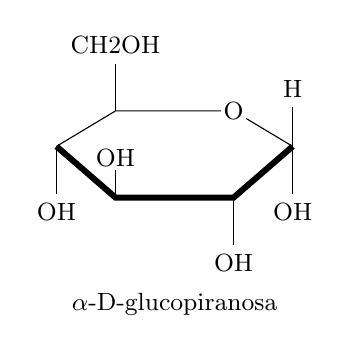
\begin{tikzpicture}[x=1cm, y=1cm, font=\small]
\coordinate (C4) at (-1.5,0); \coordinate (C3) at (-0.75,-0.65); \coordinate (C2) at (0.75,-0.65);
\coordinate (C1) at (1.5,0); \coordinate (O) at (0.75,0.45); \coordinate (C5) at (-0.75,0.45);
\draw (C5) -- (O) -- (C1); \draw (C4) -- (C5);
\draw[line width=2.2pt] (C4) -- (C3) -- (C2) -- (C1);
\node[fill=white, inner sep=1pt] at (O) {O};
\draw (C5) -- ++(0,0.6) node[above] {\ce{CH2OH}};
\draw (C1) -- ++(0,-0.6) node[below] {OH}; \draw (C1) -- ++(0,0.5) node[above] {H};
\draw (C2) -- ++(0,-0.6) node[below] {OH}; \draw (C3) -- ++(0,0.35) node[above, inner sep=1pt] {OH};
\draw (C4) -- ++(0,-0.6) node[below] {OH};
\node at (0,-2.0) {$\alpha$-D-glucopiranosa};
\end{tikzpicture}
\end{minipage}%
\begin{minipage}[c]{0.37\linewidth}\centering
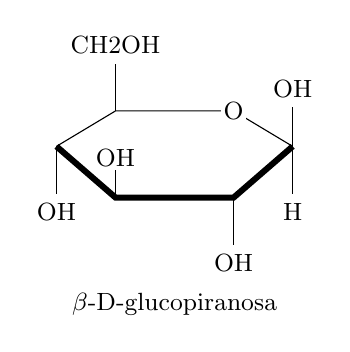
\begin{tikzpicture}[x=1cm, y=1cm, font=\small]
\coordinate (C4) at (-1.5,0); \coordinate (C3) at (-0.75,-0.65); \coordinate (C2) at (0.75,-0.65);
\coordinate (C1) at (1.5,0); \coordinate (O) at (0.75,0.45); \coordinate (C5) at (-0.75,0.45);
\draw (C5) -- (O) -- (C1); \draw (C4) -- (C5);
\draw[line width=2.2pt] (C4) -- (C3) -- (C2) -- (C1);
\node[fill=white, inner sep=1pt] at (O) {O};
\draw (C5) -- ++(0,0.6) node[above] {\ce{CH2OH}};
\draw (C1) -- ++(0,0.5) node[above] {OH}; \draw (C1) -- ++(0,-0.6) node[below] {H};
\draw (C2) -- ++(0,-0.6) node[below] {OH}; \draw (C3) -- ++(0,0.35) node[above, inner sep=1pt] {OH};
\draw (C4) -- ++(0,-0.6) node[below] {OH};
\node at (0,-2.0) {$\beta$-D-glucopiranosa};
\end{tikzpicture}
\end{minipage}
\par\vspace{6pt}

{\small La D-glucosa. Izquierda: la cadena abierta en proyección de Fischer, con el \ce{OH} de C5 a la derecha (D). Centro
y derecha: los dos \omterm{def:b2:biomolecules:anomer}{anómeros} piranosa en \omterm{def:b2:biomolecules:anomer}{proyección de Haworth}; los grupos situados a la derecha en la proyección de
Fischer apuntan hacia abajo, los de la izquierda hacia arriba, y C5 lleva el \ce{CH2OH} hacia arriba. Los \omterm{def:b2:biomolecules:anomer}{anómeros}
solo difieren en C1. Se omiten los hidrógenos de C2 a C5.}
\end{omfigure}

\begin{method}[De Fischer a Haworth (D-aldopiranosa)]\label{met:b2:biomolecules:haworth}
\begin{enumerate}
  \item Dibújese el anillo con O atrás a la derecha, C1 a la derecha, y luego C2, C3, C4 en el sentido de las agujas del reloj por
        delante y a la izquierda, con C5 atrás a la izquierda.
  \item Los grupos situados a la derecha en la proyección de Fischer van hacia abajo, y los de la izquierda, hacia arriba.
  \item En C5 (serie D), el \ce{CH2OH} va hacia arriba.
  \item En C1, el \ce{OH} va hacia abajo para $\alpha$ y hacia arriba para $\beta$.
\end{enumerate}
\end{method}

\begin{proposition}[Equilibrio de mutarrotación]\label{prop:b2:biomolecules:mutarotation}
Si las rotaciones específicas de los \omterm{def:b2:biomolecules:anomer}{anómeros} puros son $[\alpha]_\alpha$ y $[\alpha]_\beta$ y la de la
mezcla en equilibrio es $[\alpha]_{\mathrm{eq}}$, la fracción molar del anómero $\alpha$ en el
equilibrio es
\begin{equation*}
x_\alpha = \frac{[\alpha]_{\mathrm{eq}} - [\alpha]_\beta}{[\alpha]_\alpha - [\alpha]_\beta}.
\end{equation*}
\end{proposition}

\begin{proof}
La cadena abierta es una fracción ínfima de la mezcla y se desprecia. Las rotaciones de los dos \omterm{def:b2:biomolecules:anomer}{anómeros}
se suman en proporción a sus concentraciones (ley de Biot, volumen del primer año); como tienen la misma masa
molar, $[\alpha]_{\mathrm{eq}} = x_\alpha[\alpha]_\alpha + (1 - x_\alpha)[\alpha]_\beta$, que se resuelve
para $x_\alpha$.
\end{proof}

La D-glucosa en equilibrio en agua tiene $[\alpha] = +52.7$ (en \unit{\degree\,dm^{-1}\,g^{-1}\,mL}).
Con rotaciones de los \omterm{def:b2:biomolecules:anomer}{anómeros} de $+112$ y $+18.7$ (datos de ejercicio), $x_\alpha = (52.7 - 18.7)/(112 - 18.7)
\approx 0.36$: un 36~\% de $\alpha$ y un 64~\% de $\beta$, aproximadamente. El anómero $\beta$, con todos sus
sustituyentes ecuatoriales en la silla, es el más estable.
% ledger: rot:glucose-eq

\begin{definition}[Glicósidos]\label{def:b2:biomolecules:glycoside}
Un \emph{glicósido}\index{glicosido@glicósido} es el acetal que se forma cuando el \ce{OH} anomérico de un azúcar se sustituye
por un grupo \ce{OR} procedente de un alcohol, a menudo otro azúcar; el enlace del \omterm{def:b2:biomolecules:anomer}{carbono anomérico} con ese
oxígeno es el \emph{enlace glicosídico}\index{enlace glicosidico@enlace glicosídico}. Un \emph{azúcar reductor}\index{azucar reductor@azúcar reductor}
es el que reduce oxidantes suaves como el licor de Fehling o el reactivo de Tollens.
\end{definition}

\begin{proposition}[Reductor o no]\label{prop:b2:biomolecules:reducing}
Un azúcar con un grupo hemiacetal (o hemicetal) libre es reductor; un \omterm{def:b2:biomolecules:glycoside}{glicósido} cuyos \omterm{def:b2:biomolecules:anomer}{carbonos anoméricos} están
todos comprometidos en \omterm{def:b2:biomolecules:glycoside}{enlaces glicosídicos} no lo es.
\end{proposition}

\begin{proof}[Argumento]
Un hemiacetal está en equilibrio con la cadena abierta, cuyo grupo aldehído es oxidado por el reactivo;
el equilibrio abre entonces más anillos hasta que ha reaccionado todo el azúcar. Un acetal no se abre en
agua neutra o básica: el \omterm{def:b2:biomolecules:anomer}{carbono anomérico} queda bloqueado, sin aldehído que oxidar.
\end{proof}

La maltosa (dos glucosas, el C1 de una unido al O4 de la otra) conserva un hemiacetal libre y es reductora;
la sacarosa une entre sí los \omterm{def:b2:biomolecules:anomer}{carbonos anoméricos} de la glucosa y de la fructosa y no lo es. El almidón y la
celulosa son ambos cadenas de glucosa unidas C1--O4: $\alpha$ en el almidón, que se enrolla y se digiere;
$\beta$ en la celulosa, cuyas cadenas rectas se empaquetan en fibras unidas por enlaces de hidrógeno.

\section{Lípidos}

\begin{definition}[Lípidos]\label{def:b2:biomolecules:lipid}
Un \emph{ácido graso}\index{acido graso@ácido graso} es un ácido carboxílico de cadena larga no ramificada, normalmente de 12 a
22 carbonos, saturada o con dobles enlaces (\textit{Z}). Un \emph{triglicérido}\index{triglicerido@triglicérido} es el
triéster del propano-1,2,3-triol (glicerol) con tres ácidos grasos. Un
\emph{fosfolípido}\index{fosfolipido@fosfolípido} es un diéster del glicerol con dos ácidos grasos cuya tercera
posición lleva un grupo fosfato unido a un pequeño grupo polar.
\end{definition}

Los dobles enlaces (\textit{Z}) doblan las cadenas, que entonces se empaquetan mal: el ácido esteárico (18 carbonos,
saturado) funde a \qty{69}{\degreeCelsius}, y el ácido oleico (18 carbonos, un doble enlace \textit{Z}), a
\qty{13}{\degreeCelsius}. Las grasas ricas en cadenas saturadas son sólidas a temperatura ambiente; los aceites, ricos en
cadenas insaturadas, son líquidos. Los \omterm{def:b2:biomolecules:lipid}{triglicéridos} se saponifican en glicerol y jabones
(\cref{ch:b2:acyl-substitution}).
% ledger: mp:stearic, mp:oleic

\begin{omfigure}
\begin{tikzpicture}[x=1cm, y=1cm]
\foreach \i in {0,1,2,3,4,5,6,7,8,9}{
  \fill[omDef!60] (0.6*\i,1.6) circle (0.17);
  \draw[thick, black!70] (0.6*\i-0.06,1.43) .. controls (0.6*\i-0.12,1.2) and (0.6*\i,1.0) .. (0.6*\i-0.06,0.75);
  \draw[thick, black!70] (0.6*\i+0.06,1.43) .. controls (0.6*\i+0.12,1.2) and (0.6*\i,1.0) .. (0.6*\i+0.06,0.75);
  \fill[omDef!60] (0.6*\i,-0.6) circle (0.17);
  \draw[thick, black!70] (0.6*\i-0.06,-0.43) .. controls (0.6*\i-0.12,-0.2) and (0.6*\i,0.0) .. (0.6*\i-0.06,0.25);
  \draw[thick, black!70] (0.6*\i+0.06,-0.43) .. controls (0.6*\i+0.12,-0.2) and (0.6*\i,0.0) .. (0.6*\i+0.06,0.25);
}
\node[font=\small, anchor=west] at (6.0,2.2) {agua};
\node[font=\small, anchor=west] at (6.0,0.5) {núcleo hidrocarbonado};
\node[font=\small, anchor=west] at (6.0,-1.2) {agua};
\draw[densely dotted] (5.6,1.6) -- (6.0,1.6) node[right, font=\footnotesize] {cabezas polares};
\draw[densely dotted] (5.6,1.05) -- (6.0,1.05) node[right, font=\footnotesize] {dos colas de ácido graso};
\end{tikzpicture}
\par\vspace{4pt}

{\small Una bicapa de \omterm{def:b2:biomolecules:lipid}{fosfolípidos}, esquema: las cabezas polares miran al agua por ambos lados, y las
colas hidrocarbonadas se encuentran en el interior. Las membranas celulares se construyen sobre esta estructura; los jabones,
con una cola por cabeza, forman en cambio pequeñas esferas con las colas en el interior, llamadas micelas.}
\end{omfigure}

\section{Nucleótidos}

\begin{definition}[Nucleótidos]\label{def:b2:biomolecules:nucleotide}
Una \emph{base nitrogenada}\index{base nitrogenada} es un heterociclo nitrogenado: la adenina (A) y la guanina (G), purinas;
la citosina (C), la timina (T) y el uracilo (U), pirimidinas. Un \emph{nucleósido}\index{nucleosido@nucleósido} es una
base nitrogenada unida por un nitrógeno al C1 de la ribosa o de la 2-desoxirribosa (un $N$-glicósido). Un
\emph{nucleótido}\index{nucleotido@nucleótido} es un éster fosfórico de un nucleósido. En los ácidos nucleicos los
nucleótidos están unidos por \emph{enlaces fosfodiéster}\index{enlace fosfodiester@enlace fosfodiéster}: un fosfato une
el O3 de un azúcar con el O5 del siguiente.
\end{definition}

El ADN usa 2-desoxirribosa y las bases A, G, C, T; el ARN usa ribosa y U en lugar de T. La cadena tiene un
sentido, de su extremo 5$'$ a su extremo 3$'$, y los fosfatos, ionizados a pH fisiológico, la convierten en un
polianión. Dos hebras de ADN discurren en sentidos opuestos y se mantienen unidas por enlaces de hidrógeno entre
bases enfrentadas.

\begin{proposition}[Apareamiento de bases]\label{prop:b2:biomolecules:pairing}
En el ADN bicatenario, la adenina se aparea con la timina mediante dos enlaces de hidrógeno, y la guanina con la citosina
mediante tres.
\end{proposition}

\begin{proof}[Argumento]
Los pares son aquellos cuyos bordes hacen coincidir dadores (\ce{N-H}) con aceptores (oxígeno de \ce{C=O}, nitrógeno
del anillo) a las distancias adecuadas, con una purina frente a una pirimidina para que todos los pares tengan la misma
anchura. A ofrece \ce{N-H} (su grupo amino) y un \ce{N} del anillo; T ofrece \ce{C=O} y \ce{N-H}: dos enlaces. G
ofrece \ce{C=O}, \ce{N-H} y \ce{N-H} (amino); C ofrece \ce{N-H} (amino), \ce{N} y \ce{C=O}: tres
enlaces. La figura los muestra.
\end{proof}

\begin{omfigure}
\setchemfig{atom sep=1.7em}
\chemfig{?[a](-[:90]CH_3)-[:-30](=[:30]@{to}O)-[:-90]N(-[:-30]@{th}H)-[:-150](=[:-90]O)-[:150]N(-[:-150]R)-[:90]?[a,2]}%
\hspace{2.3em}%
\raisebox{-1.0em}{\chemfig{?[a](-[:150]N(-[:90]H)-[:210]@{ah}H)-[:30]?[b](-[:78]N=[:6]-[:-66]N(-[:-30]R)-[:-138]?[c])=[:-30]?[c]-[:-90]N=[:-150]-[:150]@{an}N?[a,2]}}
\chemmove{\draw[-, densely dotted, thick](to)--(ah); \draw[-, densely dotted, thick](th)--(an);}
\hspace{1.5em}
\chemfig{?[a]-[:-30](-[:30]N(-[:90]H)-[:-30]@{ch}H)=[:-90]@{cn}N-[:-150](=[:-90]@{co}O)-[:150]N(-[:-150]R)-[:90]?[a,2]}%
\hspace{2.3em}%
\raisebox{-0.6em}{\chemfig{?[a](=[:150]@{go}O)-[:30]?[b](-[:78]N=[:6]-[:-66]N(-[:-30]R)-[:-138]?[c])=[:-30]?[c]-[:-90]N=[:-150](-[:-90]N(-[:-30]H)-[:-150]@{gh}H)-[:150]N?[a](-[:180]@{gn}H)}}
\chemmove{\draw[-, densely dotted, thick](ch)--(go); \draw[-, densely dotted, thick](cn)--(gn);
  \draw[-, densely dotted, thick](co)--(gh);}
\par\vspace{6pt}

{\small Los dos pares de bases del ADN. Izquierda: timina y adenina, dos enlaces de hidrógeno (punteados). Derecha:
citosina y guanina, tres. R es la desoxirribosa de cada hebra; los dos grupos R de un par apuntan hacia el
mismo lado, hacia los dos esqueletos.}
\end{omfigure}

\begin{history}[Los azúcares, 1891]
\begin{minipage}[t]{0.18\linewidth}
\vspace{0pt}
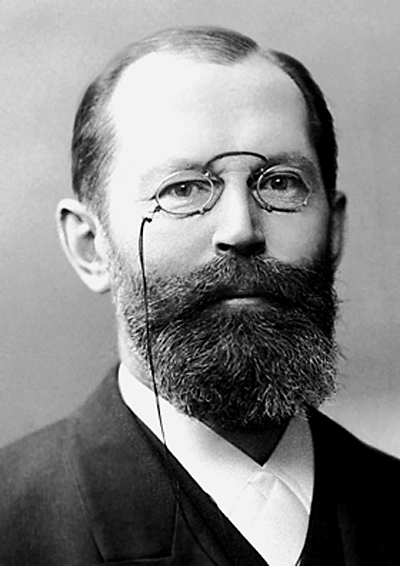
\includegraphics[width=\linewidth]{images/book3/fischer.jpg}
\end{minipage}\hfill
\begin{minipage}[t]{0.78\linewidth}
\vspace{0pt}
Emil Fischer estableció, hacia 1891, las configuraciones de la glucosa y de sus isómeros, antes de que ningún
método físico pudiera ver una molécula: convirtiendo unos azúcares en otros y contando los
estereoisómeros obtenidos. La proyección que inventó para escribirlos aún lleva su nombre. Preparó también
los primeros \omterm{def:b2:biomolecules:peptide}{péptidos} sintéticos, y recibió el Premio Nobel de Química de 1902. (Retrato: Atelier
Victoria, Berlín, hacia 1895, dominio público; Wikimedia Commons.)
\end{minipage}
\end{history}

\section{Ejercicios}

\begin{exercise}[$\star$]\label{exo:b2:biomolecules:1}
Dibújese la alanina como \omterm{def:b2:biomolecules:amino-acid}{ion dipolar}, y luego las formas que predominan a pH 1 y a pH 12.
\end{exercise}

\begin{exercise}[$\star$]\label{exo:b2:biomolecules:2}
Calcúlese el \omterm{def:b2:biomolecules:amino-acid}{punto isoeléctrico} de la glicina, y el de la alanina ($\mathrm pK_a$ 2.35 y 9.87).
\end{exercise}

\begin{exercise}[$\star$]\label{exo:b2:biomolecules:3}
Dibújese el dipéptido Ala--Gly y rodéese con un círculo su \omterm{def:b2:biomolecules:peptide}{enlace peptídico}. ¿En qué se diferencia de Gly--Ala?
\end{exercise}

\begin{exercise}[$\star$]\label{exo:b2:biomolecules:4}
En una proyección de Fischer con el \ce{COOH} arriba y la \omterm{def:b2:biomolecules:amino-acid}{cadena lateral} \ce{CH2OH} abajo, el
\ce{NH2} de la serina apunta a la izquierda. ¿Es D o L? Dese su descriptor CIP.
\end{exercise}

\begin{exercise}[$\star\star$]\label{exo:b2:biomolecules:5}
Dese la carga neta del tripéptido Lys--Gly--Asp a pH 1, 7 y 12.
\end{exercise}

\begin{exercise}[$\star\star$]\label{exo:b2:biomolecules:6}
¿Por qué se usa un \omterm{def:b2:biomolecules:peptide}{agente de acoplamiento} para formar un \omterm{def:b2:biomolecules:peptide}{enlace peptídico}, en lugar de un \omterm{def:b2:acyl-substitution:derivative}{cloruro de acilo} del aminoácido
protegido preparado con cloruro de tionilo y calentado?
\end{exercise}

\begin{exercise}[$\star\star$]\label{exo:b2:biomolecules:7}
La D-fructosa se cicla a través del \ce{OH} de su C5 sobre la cetona de C2. Indíquese el tamaño del anillo y dibújese la
$\beta$-D-fructofuranosa en \omterm{def:b2:biomolecules:anomer}{proyección de Haworth}.
\end{exercise}

\begin{exercise}[$\star\star$]\label{exo:b2:biomolecules:8}
Los \omterm{def:b2:biomolecules:anomer}{anómeros} puros de la D-galactosa tienen rotaciones específicas de $+150.7$ ($\alpha$) y $+52.8$ ($\beta$), y
la mezcla en equilibrio, $+80.2$ (datos de ejercicio). Calcúlese la composición en el equilibrio.
\end{exercise}

\begin{exercise}[$\star\star$]\label{exo:b2:biomolecules:9}
Explíquese por qué la maltosa reduce el licor de Fehling y la sacarosa no, y por qué la sacarosa sí lo hace tras
calentarla con ácido diluido.
\end{exercise}

\begin{exercise}[$\star\star\star$]\label{exo:b2:biomolecules:10}
El índice de \omterm{def:b2:acyl-substitution:saponification}{saponificación} de una grasa es la masa de hidróxido de potasio, en mg, que saponifica 1~g de ella.
Calcúlese para la trioleína, \ce{C57H104O6}, y explíquese por qué una grasa de cadenas más cortas tiene un valor más alto.
\end{exercise}

\begin{exercise}[$\star\star\star$]\label{exo:b2:biomolecules:11}
Planifíquese la síntesis de Gly--Ala a partir de glicina y alanina: grupos protectores, activación, acoplamiento,
desprotección, con un par ortogonal.
\end{exercise}

\begin{exercise}[$\star\star\star$]\label{exo:b2:biomolecules:12}
Escríbase la hebra complementaria de 5$'$-ATGCGT-3$'$, a partir de su extremo 5$'$, y cuéntense los enlaces de hidrógeno
que mantienen unida la doble hebra.
\end{exercise}

\section{Problema: el aspartamo}

\begin{problem}[{Problema de fin de semana --- los dos aminoácidos y sus configuraciones, la carga del
dipéptido en función del pH, su síntesis y el problema $\alpha$/$\beta$, y su hidrólisis en un
refresco}]
\label{pb:b2:biomolecules:1}
El aspartamo es el éster metílico del dipéptido formado por el grupo $\alpha$-carboxílico del ácido L-aspártico
con el grupo amino de la L-fenilalanina. Datos: $\mathrm pK_a$ del ácido aspártico 2.0, 3.9 y 9.9 (valores
modelo para los grupos del dipéptido). Masas molares (\unit{g/mol}): C 12.011, H 1.008, N 14.007,
O 15.999.
% ledger: use:aspartame, pka:asp1, pka:asp2, pka:asp3, aw:C, aw:H, aw:N, aw:O

\medskip
\noindent\textbf{Parte I --- Los dos aminoácidos.}
\begin{enumerate}
  \item Nómbrense los tres compuestos que libera la hidrólisis completa del aspartamo.
  \item Dibújense el ácido L-aspártico y la L-fenilalanina en proyección de Fischer.
  \item Dese el descriptor CIP de cada estereocentro.
  \item ¿Cuántos estereoisómeros tiene el aspartamo?
  \item Dibújese el aspartamo y señálense el \omterm{def:b2:biomolecules:peptide}{enlace peptídico} y el éster.
  \item ¿Por qué es importante la configuración de cada aminoácido para el sabor dulce?
\end{enumerate}

\medskip
\noindent\textbf{Parte II --- La carga en función del pH.}
\begin{enumerate}[resume]
  \item Enumérense los grupos ionizables del aspartamo. ¿Por qué el extremo C-terminal no es uno de ellos?
  \item Con los valores modelo, dese la carga neta a pH 2.
  \item Lo mismo a pH 7.
  \item Lo mismo a pH 12.
  \item Estímese el \omterm{def:b2:biomolecules:amino-acid}{punto isoeléctrico} en este modelo.
  \item ¿Por qué los verdaderos valores de $\mathrm pK_a$ del dipéptido diferirían de los del ácido aspártico
        libre?
\end{enumerate}

\medskip
\noindent\textbf{Parte III --- Síntesis.}
\begin{enumerate}[resume]
  \item ¿Por qué no pueden simplemente calentarse juntos el ácido aspártico y el éster metílico de la fenilalanina?
  \item ¿Qué grupos del ácido aspártico deben protegerse?
  \item ¿Qué le hace un \omterm{def:b2:biomolecules:peptide}{agente de acoplamiento} al grupo carboxílico libre?
  \item El ácido aspártico tiene dos grupos carboxílicos. ¿Qué se forma si se acopla el equivocado?
  \item Propóngase una protección ortogonal que deje libre solo el grupo $\alpha$-carboxílico, y su
        eliminación.
  \item ¿Por qué no debe dejarse demasiado tiempo el aminoácido activado en condiciones básicas?
  \item Escríbase la secuencia de etapas.
\end{enumerate}

\medskip
\noindent\textbf{Parte IV --- Hidrólisis en un refresco.}
\begin{enumerate}[resume]
  \item ¿Qué enlaces del aspartamo pueden hidrolizarse en una bebida ácida? ¿Cuál se rompe primero?
  \item Dense los productos de la hidrólisis del éster solo.
  \item ¿Por qué un refresco viejo sabe menos dulce?
  \item Calcúlese la masa molar del aspartamo, \ce{C14H18N2O5}.
  \item Calcúlese la cantidad de aspartamo en una lata que contiene \qty{180}{mg}.
  \item Indíquese la masa de metanol liberada por la hidrólisis completa de \qty{180}{mg} de
        aspartamo.
\end{enumerate}
\end{problem}
